\documentclass[ru]{./../../common/SurferDesc}%%%%%%%%%%%%%%%%%%%%%%%%%%%%%%%%%%%%%%%%%%%%%%%%%%%%%%%%%%%%%%%%%%%%%%%
%
% The document starts here:
%
\begin{document}
\footnotesize
% WeltrekordflŠchen

%%% 1.Tafel

%%%%%%%%%%%%%%%%%%%%%%%%%%%%%


\begin{surferPage}
  \begin{surferTitle}Октика Чмутова\end{surferTitle} \\
    На первый взгляд видно, что октика Чмутова $\text{Chm}_{d}, \ d=8,$
очень симметрична.
 Это также относительно легко можно увидеть по уравнению:
    \[\text{Chm}_{d}\colon T_d(x) + T_d(y) + T_d(z) + 1 = 0.\]
     При этом $T_d$– это т.н. многочлен Чебышёва (изображение слева). Кривая $T_8(x)+T_8(y)=0$ изображена справа:
    
     \begin{center}
      \begin{tabular}{c@{\quad}c}
        \begin{tabular}{c}
          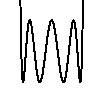
\includegraphics[height=1.75cm]{./../../common/images/Tcheb_008.pdf}
        \end{tabular}    
        &
        \begin{tabular}{c}
          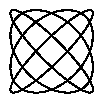
\includegraphics[height=1.75cm]{./../../common/images/Tcheb_2d_008.pdf}
        \end{tabular}    
      \end{tabular}
    \end{center}
    \vspace{-0.3cm}
От этих изображений до внешнего вида поверхности не так далеко.

Эти уравнения В. Чмутов составил в начале 80-ых годов. Тогда они представляли собой почти для всех степеней $d$ «мировой рекорд» для $\mu(d)$, т.е. максимального количества сингулярностей на поверхности степени $d$. В 90-ые годы он сам улучшил свой рекорд, а в 2005 г. С.~Бреске, О.~Лабс и Д.~ван~Стратен построили схожую конструкцию для действительных сингулярностей.

  \begin{surferText}
     \end{surferText}
\end{surferPage}
%%%%%%%%%%%%%%%%%%%%%%%%%%%%%
%%%%%%%%%%%%%%%%%%%%%%%%%%%%%


\end{document}
%
% end of the document.
%
%%%%%%%%%%%%%%%%%%%%%%%%%%%%%%%%%%%%%%%%%%%%%%%%%%%%%%%%%%%%%%%%%%%%%%%
